%%
%% This is file `sample-acmlarge.tex',
%% generated with the docstrip utility.
%%
%% The original source files were:
%%
%% samples.dtx  (with options: `acmlarge')
%% 
%% IMPORTANT NOTICE:
%% 
%% For the copyright see the source file.
%% 
%% Any modified versions of this file must be renamed
%% with new filenames distinct from sample-acmlarge.tex.
%% 
%% For distribution of the original source see the terms
%% for copying and modification in the file samples.dtx.
%% 
%% This generated file may be distributed as long as the
%% original source files, as listed above, are part of the
%% same distribution. (The sources need not necessarily be
%% in the same archive or directory.)
%%
%%
%% Commands for TeXCount
%TC:macro \cite [option:text,text]
%TC:macro \citep [option:text,text]
%TC:macro \citet [option:text,text]
%TC:envir table 0 1
%TC:envir table* 0 1
%TC:envir tabular [ignore] word
%TC:envir displaymath 0 word
%TC:envir math 0 word
%TC:envir comment 0 0
%%
%%
%% The first command in your LaTeX source must be the \documentclass
%% command.
%%
%% For submission and review of your manuscript please change the
%% command to \documentclass[manuscript, screen, review]{acmart}.
%%
%% When submitting camera ready or to TAPS, please change the command
%% to \documentclass[sigconf]{acmart} or whichever template is required
%% for your publication.
%%
%%
\documentclass[acmlarge]{acmart}
\usepackage{fontspec}
\usepackage{amsmath,amsfonts,amsthm,amssymb}
\usepackage{caption}
\usepackage{subfigure}
\usepackage{algorithmic}
\usepackage{graphicx}
\usepackage{hyperref}
\usepackage[ruled,vlined,linesnumbered]{algorithm2e}
% \usepackage[colorlinks,linkcolor=red]{hyperref}
% \usepackage{setspace}
% \usepackage{fancyhdr}
% \usepackage{lastpage}
% \usepackage{extramarks}
% \usepackage{chngpage}
% \usepackage{natbib}
% \usepackage{soul,color}
% \usepackage{color}
% \usepackage{graphicx,float,wrapfig}
% \usepackage{CJK}

\usepackage{color}
\usepackage{listings}
\lstset{ %
language=C++,                % choose the language of the code
basicstyle=\footnotesize,       % the size of the fonts that are used for the code
numbers=left,                   % where to put the line-numbers
numberstyle=\footnotesize,      % the size of the fonts that are used for the line-numbers
stepnumber=1,                   % the step between two line-numbers. If it is 1 each line will be numbered
numbersep=5pt,                  % how far the line-numbers are from the code
backgroundcolor=\color{white},  % choose the background color. You must add \usepackage{color}
showspaces=false,               % show spaces adding particular underscores
showstringspaces=false,         % underline spaces within strings
showtabs=false,                 % show tabs within strings adding particular underscores
frame=single,           % adds a frame around the code
tabsize=2,          % sets default tabsize to 2 spaces
captionpos=b,           % sets the caption-position to bottom
breaklines=true,        % sets automatic line breaking
breakatwhitespace=false,    % sets if automatic breaks should only happen at whitespace
% escapeinside={\%*}{*)}          % if you want to add a comment within your code
}

%%
%% \BibTeX command to typeset BibTeX logo in the docs
\AtBeginDocument{%
  \providecommand\BibTeX{{%
    Bib\TeX}}}

%% Rights management information.  This information is sent to you
%% when you complete the rights form.  These commands have SAMPLE
%% values in them; it is your responsibility as an author to replace
%% the commands and values with those provided to you when you
%% complete the rights form.
% \setcopyright{acmlicensed}
\copyrightyear{2024}
% \acmYear{2018}
% \acmDOI{XXXXXXX.XXXXXXX}


%%
%% These commands are for a JOURNAL article.
% \acmJournal{POMACS}
% \acmVolume{37}
% \acmNumber{4}
% \acmArticle{111}
% \acmMonth{8}

%%
%% Submission ID.
%% Use this when submitting an article to a sponsored event. You'll
%% receive a unique submission ID from the organizers
%% of the event, and this ID should be used as the parameter to this command.
%%\acmSubmissionID{123-A56-BU3}

%%
%% For managing citations, it is recommended to use bibliography
%% files in BibTeX format.
%%
%% You can then either use BibTeX with the ACM-Reference-Format style,
%% or BibLaTeX with the acmnumeric or acmauthoryear sytles, that include
%% support for advanced citation of software artefact from the
%% biblatex-software package, also separately available on CTAN.
%%
%% Look at the sample-*-biblatex.tex files for templates showcasing
%% the biblatex styles.
%%

%%
%% The majority of ACM publications use numbered citations and
%% references.  The command \citestyle{authoryear} switches to the
%% "author year" style.
%%
%% If you are preparing content for an event
%% sponsored by ACM SIGGRAPH, you must use the "author year" style of
%% citations and references.
%% Uncommenting
%% the next command will enable that style.
%%\citestyle{acmauthoryear}


%%
%% end of the preamble, start of the body of the document source.
\begin{document}

%%
%% The "title" command has an optional parameter,
%% allowing the author to define a "short title" to be used in page headers.
\title{Final Report}

%%
%% The "author" command and its associated commands are used to define
%% the authors and their affiliations.
%% Of note is the shared affiliation of the first two authors, and the
%% "authornote" and "authornotemark" commands
%% used to denote shared contribution to the research.
% \author{Ben Trovato}
% \authornote{Both authors contributed equally to this research.}
% \email{trovato@corporation.com}
% \orcid{1234-5678-9012}
% \author{G.K.M. Tobin}
% \authornotemark[1]
% \email{webmaster@marysville-ohio.com}
% \affiliation{%
%   \institution{Institute for Clarity in Documentation}
%   \streetaddress{P.O. Box 1212}
%   \city{Dublin}
%   \state{Ohio}
%   \country{USA}
%   \postcode{43017-6221}
% }

% \author{Lars Th{\o}rv{\"a}ld}
% \affiliation{%
%   \institution{The Th{\o}rv{\"a}ld Group}
%   \streetaddress{1 Th{\o}rv{\"a}ld Circle}
%   \city{Hekla}
%   \country{Iceland}}
% \email{larst@affiliation.org}

% \author{Valerie B\'eranger}
% \affiliation{%
%   \institution{Inria Paris-Rocquencourt}
%   \city{Rocquencourt}
%   \country{France}
% }

% \author{Aparna Patel}
% \affiliation{%
%  \institution{Rajiv Gandhi University}
%  \streetaddress{Rono-Hills}
%  \city{Doimukh}
%  \state{Arunachal Pradesh}
%  \country{India}}

\author{Xin Zhou}
\affiliation{%
  \institution{Tsinghua University}
  % \streetaddress{30 Shuangqing Rd}
  \city{Haidian Qu}
  \state{Beijing Shi}
  \country{China}}

% \author{Charles Palmer}
% \affiliation{%
%   \institution{Palmer Research Laboratories}
%   \streetaddress{8600 Datapoint Drive}
%   \city{San Antonio}
%   \state{Texas}
%   \country{USA}
%   \postcode{78229}}
% \email{cpalmer@prl.com}

% \author{John Smith}
% \affiliation{%
%   \institution{The Th{\o}rv{\"a}ld Group}
%   \streetaddress{1 Th{\o}rv{\"a}ld Circle}
%   \city{Hekla}
%   \country{Iceland}}
% \email{jsmith@affiliation.org}

% \author{Julius P. Kumquat}
% \affiliation{%
%   \institution{The Kumquat Consortium}
%   \city{New York}
%   \country{USA}}
% \email{jpkumquat@consortium.net}

%%
%% By default, the full list of authors will be used in the page
%% headers. Often, this list is too long, and will overlap
%% other information printed in the page headers. This command allows
%% the author to define a more concise list
%% of authors' names for this purpose.
% \renewcommand{\shortauthors}{Trovato et al.}

%%
%% The abstract is a short summary of the work to be presented in the
%% article.
% \begin{abstract}
%   A clear and well-documented \LaTeX\ document is presented as an
%   article formatted for publication by ACM in a conference proceedings
%   or journal publication. Based on the ``acmart'' document class, this
%   article presents and explains many of the common variations, as well
%   as many of the formatting elements an author may use in the
%   preparation of the documentation of their work.
% \end{abstract}

%%
%% The code below is generated by the tool at http://dl.acm.org/ccs.cfm.
%% Please copy and paste the code instead of the example below.
%%
% \begin{CCSXML}
% <ccs2012>
%  <concept>
%   <concept_id>00000000.0000000.0000000</concept_id>
%   <concept_desc>Do Not Use This Code, Generate the Correct Terms for Your Paper</concept_desc>
%   <concept_significance>500</concept_significance>
%  </concept>
%  <concept>
%   <concept_id>00000000.00000000.00000000</concept_id>
%   <concept_desc>Do Not Use This Code, Generate the Correct Terms for Your Paper</concept_desc>
%   <concept_significance>300</concept_significance>
%  </concept>
%  <concept>
%   <concept_id>00000000.00000000.00000000</concept_id>
%   <concept_desc>Do Not Use This Code, Generate the Correct Terms for Your Paper</concept_desc>
%   <concept_significance>100</concept_significance>
%  </concept>
%  <concept>
%   <concept_id>00000000.00000000.00000000</concept_id>
%   <concept_desc>Do Not Use This Code, Generate the Correct Terms for Your Paper</concept_desc>
%   <concept_significance>100</concept_significance>
%  </concept>
% </ccs2012>
% \end{CCSXML}

% \ccsdesc[500]{Do Not Use This Code~Generate the Correct Terms for Your Paper}
% \ccsdesc[300]{Do Not Use This Code~Generate the Correct Terms for Your Paper}
% \ccsdesc{Do Not Use This Code~Generate the Correct Terms for Your Paper}
% \ccsdesc[100]{Do Not Use This Code~Generate the Correct Terms for Your Paper}

%%
%% Keywords. The author(s) should pick words that accurately describe
%% the work being presented. Separate the keywords with commas.
% \keywords{Do, Not, Us, This, Code, Put, the, Correct, Terms, for,
%   Your, Paper}

% \received{20 February 2007}
% \received[revised]{12 March 2009}
% \received[accepted]{5 June 2009}

%%
%% This command processes the author and affiliation and title
%% information and builds the first part of the formatted document.
\maketitle

\section{Introduction}

My project mainly reproduces 
the paper ``Interlinked SPH Pressure Solvers for Strong Fluid-Rigid Coupling"\cite{2019TOG} .
% TODO: add citation
The following content of this report consists of several sections: Method, Implementation, Result, Discussion, 
Personal Feeling, References.

In the Method section, first I will review
the principle of SPH and introduce the IISPH algorithm.
Then
I will introduce the algorithm overview of the
SPH-based strong fluid-rigid coupling.

In the Implementation section, I will introduce simulator structure,
scene generator and render structure, and acceleration structure.
In the end of this section, I will also talk about some problems I met in the debugging.

In the result section, I will show the video results and acceleration effect of my simulator.

In the discussion section, I will discuss some problems about this paper 
combining my experience in reproducing this paper.

In the last two sections, just like the section names,
the contents are my personal feeling and the references.

I am the only one in my team, and all the work is done by myself. So there is no 
Personal Contribution section. But the external tools I used are listed in the report.
% Personal Contribution is ignored

\section{Method}

The following content is just an overview, not covering all details.

Some of the following contents refers to the tutorial 
``Smoothed Particle Hydrodynamics Techniques for the Physics Based Simulation of Fluids and Solids"\cite{SPH-Intro}.
% TODO: add citation
It's a good tutorial for SPH. It helps me a lot.

\subsection{Basic SPH}

The main idea of SPH is to approximate the field by a finite set of simple kernel functions.
All field information including density, pressure, force, are represeted as a collection of particles.

Specifically, a common choice for the kernel function is the cubic spline kernel.
With a given collection of particles, their positions $x_1,x_2,\cdots,x_n$, their masses $m_1,m_2,\cdots,m_n$,
the density of a particle $i$ is calculated by
\begin{align}
  \rho_i=\sum_j m_j W(x_i-x_j,h)
\end{align}
Similarly, for certain field $A_i$ evaluating on the given collection of particles, 
the differential operators on $A_i$ can be approximated as:
\begin{align}
  \nabla A_i &\approx \rho_i \sum_j m_j (\frac{A_i}{\rho_i^2}+\frac{A_j}{\rho_j^2})\nabla_i W(x_i-x_j,h)\\
  \nabla^2 A_i &\approx -\sum_j \frac{m_j}{\rho_j}(A_i-A_j)\frac{2\Vert \nabla_i W(x_i-x_j,h) \Vert}{\Vert x_i-x_j \Vert}
\end{align}

According to the paper ``Weakly Compressible SPH for Free Surface Flows''\cite{WCSPH},
%TODO: add citation
the pressure field can be calculated by
\begin{align}
  P=B((\frac{\rho}{\rho_0})^\gamma-1)
\end{align}
where $B$ is a pressure constant, $\gamma=7$, $\rho_0$ is the rest density of the fluid.

Thus, we can obtain a simple fluid simulator using the above SPH method and symplectic Euler integration:
\floatname{algorithm}{}
\begin{algorithm}[!h]
  \caption{Simple Simulator}
  \ForEach{particle $i$ }{
    Reconstruct density $\rho_i$ at $x_i$ using Eq. (1) \;
  }
  \ForEach{particle $i$ }{
    Compute the viscosity force $F_i^{viscosity}=m_i \mu \nabla^2v_i  $ using Eq. (3) \;
    $v_i^*=v_i+\frac{\Delta t}{m_i}(F_i^{viscosity}+F_i^{external})$ where $F_i^{external}$ means the external force like gravity \;
  }
  Compute the pressure field $p_i$ at each particle using Eq. (4) \;
  \ForEach{particle $i$ }{
    Compute the pressure force $F_i^{pressure}=-\frac{1}{\rho}\nabla p $ using Eq. (2) \;
  }
  \ForEach{particle $i$ }{
    $v_i(t+\Delta t)=v_i^*+\frac{\Delta t}{m_i}F_i^{pressure}$ \;
    $x_i(t+\Delta t)=x_i+\Delta t v_i(t+\Delta t)$ \;
  }
\end{algorithm}

\subsection{IISPH}
IISPH is so called ``Implicit Incompressible SPH''\cite{IISPH}. 
%TODO: add citation

The theoretical foundation of IISPH is the Continuity Equation:
\begin{align*}
  \frac{\partial \rho}{\partial t}+\rho(\nabla \cdot  v)=0
\end{align*}
% We know that fluids are Incompressible materials, so 
% \begin{align*}
%   \frac{\partial \rho}{\partial t}=0 \Leftrightarrow \nabla \cdot v=0
% \end{align*}
% The main idea is to s

In the following we will use $W_{ij}$ as an simplification notation of $W(x_i-x_j,h)$.

Considering all non-pressure accelerations $v^*=v(t)+\Delta t a^{nonp}(t)$, we can 
use the continuity equation to estimate a predicted density $\rho^*=\rho(t)-\Delta t\rho(t)\nabla\cdot v^*$.
Then, we need to find a pressure acceleration $-\frac{1}{\rho(t)}\nabla p(t)$.
This acceleration leads to a velocity change $-\Delta t\frac{1}{\rho(t)}\nabla p(t)$ whose divergence 
is $-\rho(t)\nabla \cdot (\Delta t\frac{1}{\rho(t)}\nabla p(t))$ that can cancel the predicted density deviation 
$\frac{\rho_0-\rho^*}{\Delta t}$
due to non-pressure accelerations, i.e. $\frac{\rho_0-\rho^*}{\Delta t}-\rho(t)\nabla \cdot (\Delta t\frac{1}{\rho(t)}\nabla p(t))=0$.
The two kinds of density deviation should be able to be cancelled out because fluids are imcompressible materials which means
$\frac{\partial \rho}{\partial t}=0$.

Thus we get one form of a Pressure Poisson Equation which can be written as 
\begin{align*}
  \Delta t^2\nabla^2 p_i=\rho_0-\rho_i^*
\end{align*}

Using SPH, the right side can be simplified as 
\begin{align*}
  \rho_0-\rho_i^*=\rho_0-\rho_i-\Delta t\sum_j m_j (v_i^*-v_j^*)\cdot \nabla W_{ij}
\end{align*}
where $v_i^*=v_i+\Delta t a_i^{nonp}$.
The left side can be simplified as
\begin{align*}
  \Delta t^2\nabla^2 p_i&=-\Delta t \rho_i\nabla\cdot(\Delta t a_i^p)\\
  &=\Delta t^2\sum_j m_j (a_i^p-a_j^p)\cdot  W_{ij}
\end{align*}
with pressure acceleration
\begin{align*}
  a_i^p=-\frac{1}{\rho_i}\nabla p_i=-\sum_j m_j(\frac{p_i}{\rho_i^2}+\frac{p_j}{\rho_j^2})\nabla W_{ij} 
\end{align*}

Hence, we get equations whose unknown elements are $p_i$:
\begin{align*}
  \Delta t^2\sum_j m_j (a_i^p-a_j^p)\cdot  W_{ij}=\rho_0-\rho_i^*
\end{align*}
We can write it as linear equations $(Ap)_i=s_i$, where 
\begin{align*}
  (Ap)_i=\Delta t^2\sum_j m_j (a_i^p-a_j^p)\cdot  W_{ij}\\
  s_i=\rho_0-\rho_i^*
\end{align*}
Solving this linear system to get pressure in each time step instead of directly using Eq. (4), we get IISPH.

This linear system is very sparse, so we can use Relaxed Jacobi scheme instead of naive Gaussian Elimination. Specifically, 
we can use the following iteration to solve the linear system:
\begin{align*}
  p_i^{(k+1)}&=\omega\frac{s_i-\sum_{j\neq i}A_{ij}p_j^{(k)}}{A_{ii}}+(1-\omega)p_i^{(k)}\\
  &=p_i^{(k)}+\frac{\omega}{A_{ii}}(s_i-(Ap^{(k)})_i)
\end{align*}

\subsection{Strong Fluid-Rigid Coupling}

Now, with the groundwork ahead, we can talk about the main paper\cite{2019TOG}.
%TODO: add citation

The theoretical foundation of this work is still the Continuity Equation. However, the 
concept is extended to rigid body. The continuity equation is used to derive both the fluid pressure forces 
and rigid-rigid contact forces.

The rigid body is also represented by particles just like the fluid.
Discretizing the continuity equation $\frac{\partial \rho}{\partial t}+\rho_r(\nabla \cdot  v_r)=0$ for rigid particles $r$, we get 
\begin{align}
  \frac{\rho_r^0-\rho_r}{\Delta t}=-\nabla \cdot v_r^{next}
\end{align}
where $\frac{\partial \rho}{\partial t}$ is discretized by backward difference and $\rho_r^{next}$ is replaced by $\rho_r^0$ because 
imcompressiblility.

By rigid body dynamics, we have
\begin{align}
  v_r^{next}=v_R^{next}+\omega_R^{next}\times r_r^{next}
\end{align}
where $v_R^{next}$ and $\omega_R^{next}$ are the linear and angular velocity of the rigid body $R$ containing $r$, 
$r_r^{next}$ is the vector from the center of mass of the rigid body $R$ to the rigid particle $r$.

Using Euler integration and Newton's second law, we have
\begin{align}
  v_R^{next}=v_R+\Delta t\frac{1}{M_R}(F_R+\sum_k F_k^{rr})\\
  \omega_R^{next}=\omega_R+\Delta t I_R^{-1}(\tau_R+(I_R\omega_R)\times\omega_R+ \sum_k r_k\times F_k^{rr})
\end{align}
where $M_R$ means the mass of the rigid body $R$, $I_R$ means the inertia tensor of the rigid body $R$,
$F_R$ and $\tau_R$ means the external force and torque on the rigid body $R$ including gravity and 
fluid-rigid interface forces, $F_k^{rr}$ means the unknown rigid-rigid contact forces.
Using Newton's third law, Fluid-rigid interface forces can be 
obtained by the reaction forces of pressure forces from the rigid bodies to fluids
which are computed similarly to fluid pressure forces.


\floatname{algorithm}{Main Algorithm}
\begin{algorithm}[!h]
  \caption{Main Algorithm\label{MA}}
  Initialize $l$=0, $\rho_f^l,\rho_r^l,v_f^{*,l},v_r^{*,l} $ \;
  \While{ Density deviation too large }{
    Compute fluid pressure forces $F_f^{p,l+1}(p_f^l)$ \;
    Compute predicted fluid velocity $v_f^{*,l+1}(F_f^{p,l+1})$ \;
    Compute fluid-rigid interface forces $F_r^{fr,l+1}(p_f^l)$ \;
    Compute source term $s_r^{l+1} (F_r^{fr,l+1}) $ \;
    Compute rigid-rigid contact forces $F_r^{rr,l+1}=-V_r\nabla p_r^l $ \;
    Compute predicted rigid velocity $v_r^{*,l+1}=v_r^{s,l+1}+v_r^{rr,l+1} $ \;
    Compute pressure $p_r^{l+1},p_f^{l+1} $ \;
    $l$ += $1$ \;
  }
  Update fluid and rigid bodies \;
\end{algorithm}

Substitute Eq. (6), Eq. (7), Eq. (8) into Eq. (5), we get
\begin{align*}
  \frac{\rho_r^0-\rho_r}{\Delta t}=
  &-\rho_r\nabla \cdot (v_R+\Delta t\frac{1}{M_R}F_R)-\rho_r\nabla \cdot (\Delta t\frac{1}{M_R}\sum_k F_k^{rr})\\
  &-\rho_r\nabla \cdot ((\omega_R+I_R^{-1}(\Delta t\tau_R+\Delta t(I_R\omega_R)\times\omega_R))\times r_r^{next})\\
  &-\rho_r\nabla \cdot (\Delta t (I_R^{-1}\sum_k r_k\times F_k^{rr})\times r_r^{next})
\end{align*}
Introduce the approximation $r_r^{next}=r_r$ and the term $s_r$ with $s_r=\frac{\rho_r^0-\rho_r}{\Delta t}+\rho_r\nabla\cdot v_r^s $
with $v_r^s=v_R+\Delta t\frac{1}{M_R}F_R+(\omega_R+I_R^{-1}(\Delta t\tau_R+\Delta t(I_R\omega_R)\times\omega_R))\times r_r^{next} $.

Thus we can rewrite the above equation as 
\begin{align*}
  s_r=-\rho_r\nabla \cdot (\Delta t\frac{1}{M_R}\sum_k F_k^{rr}-(\Delta t I_R^{-1}\sum_k r_k\times F_k^{rr})\times r_r)
\end{align*}
which can be written as 
\begin{align*}
  s_r=-\rho_r\nabla\cdot(\Delta t\sum_k K_{rk}F_k^{rr})
\end{align*}
with $K_{rk}=\frac{1}{M_R}\mathbb{I}-\tilde{r_r}I_R^{-1}\tilde{r_k} $ where $\tilde{r}$ means 
the skew-symmetric cross-product matrix of $r$ and $\mathbb{I}$ means the identity matrix.

We model the rigid-rigid contact forces as pressure forces, i.e. $F_k^{rr}=-V_k\nabla p_k$ where $V_k$ is an 
artificial volume of the rigid particle $k$ and $p_k$ is an unknown artificial pressure. Then we get
\begin{align*}
  s_r=\rho_r\nabla\cdot(\Delta t\sum_k V_k K_{rk}\nabla p_k)
\end{align*}

Just like what we do in IISPH, similarly we use relaxed Jacobi scheme again to solve the linear system and 
get the unknown artificial pressure $p_k$ for rigid particles. And the iteration of fluid pressure $\rho_f$ and rigid pressure $\rho_r$
are doned synchronously like the pseudo code in the Main Algorithm\ref{MA}. That's why it's called strong fluid-rigid coupling.



\section{Implementation}

\subsection{Simulator Structure}

The code mentioned in this subsection is all in the file \texttt{sim.cpp}.

The main simulation loop is implemented in the function \texttt{step()}.

There are so many Neighborhood Search operations in the algorithm, so I abstract it as a function with template
\begin{lstlisting}
  template<typename T>inline void for_neighbor()
\end{lstlisting}
The type $T$ passed to the function is a \texttt{struct} with four member functions:
\begin{lstlisting}
	inline bool check(int i); // check if particle i is considered in this search
	inline void init(int i); // initialize the information
	inline void update(int i,int j); // update the information when particle i and j are detected to be neighbors
	inline void finish(int i); // use the gathered information to do something
\end{lstlisting}

Before starting Jacobi iteration, we need to initialize the linear system. I run $\texttt{for\_neighbor<update\_rho>()}$ to 
reconstruct the density of each particle. 
Then I run $\texttt{for\_neighbor<update2>()}$ and $\texttt{for\_neighbor<update3>()}$
to compute the non-pressure forces, new velocities due to non-pressure forces, 
the coefficients $A_{ii}$ and $s_i$ required by IISPH for fluid particles.
Then I manually run a neighborhood search to compute the coefficients $A_{ii}$ for rigid particles.

In the Jacobi iteration, I run $\texttt{for\_neighbor<update\_fluid\_pressure\_force>()}$ like line 3 in the Main Algorithm\ref{MA}.

Then I run $\texttt{for\_neighbor<update\_s>()}$ like line 6 in the Main Algorithm\ref{MA}.

Then I run $\texttt{for\_neighbor<update\_rigid\_pressure\_force>()}$ like line 7 in the Main Algorithm\ref{MA}.

Then I run $\texttt{for\_neighbor<update4>()}$ to update pressures and check if the average error is small enough to stop the iteration.
If the number of Jacobi iteration steps has been too many, I also stop it.

After obtaining the pressure, I recompute the pressure forces, update linear velocities and angular velocities of rigid bodies,
and then update particles.

\subsection{Scene Generator and Render Structure}

The code mentioned in this subsection is put under the directories \texttt{scene} and \texttt{render}.

Compile and run \texttt{scene1.cpp} or \texttt{scene2.cpp} or \texttt{scene3.cpp}, it will generate a file \texttt{scene.txt} as the input for the simulator.
The scene generators only contain simple geometry now. In \texttt{scene.txt}, all rigid bodies are represented by particles which are uniformly sampled inside 
the geometry. The moment of inertia of each rigid body is also computed by the chosen sample particles(to avoid tedious integration computation).
Each rigid body and each particle will start to appear in the scene at a frame specified in \texttt{scene.txt}.

Then run \texttt{b.py}, it will generate \texttt{tmp2/output*.obj} describing the mesh representations of each rigid body by running 
surface reconstruction tool on given rigid particles.

Then run simulator, it will generate the position of each particle, the center of mass of each rigid body,
the rotation of each rigid body relative to its center of mass(in matrix format),
at each frame. These files are put in \texttt{raw/*}.

\texttt{render.py} is a simple render using taichi. Its speed is fast enough for debugging. But its rendering quality is not so good.

$\texttt{gen\_fluid.py}$ runs surface reconstruction tool on fluid particles to generate the mesh representation of fluid for each frame.
$\texttt{gen\_rigid.cpp}$ generates the mesh representations of rigid bodies for each frame according to their positions of center of mass and their rotation matrices.

The surface reconstruction tool I used is \href{https://github.com/InteractiveComputerGraphics/splashsurf}{splashsurf} \cite{LBJB23}.

Then I use Blender to render the scene like \href{https://blog.csdn.net/weixin_43940314/article/details/125260073}{this tutorial}.
% TODO: add citation
In this tutorial, objects are imported as mesh sequences. It's difficulty to distinguish two rigid bodies in the same 
mesh sequence and color them respectively. So I place objects with different colors 
in different mesh sequences in advance when generating mesh representations.

\subsection{Acceleration}

In this subsection, I will talk about acceleration techniques I used in my simulator.

\subsubsection{Algorithm Acceleration}
I use the classic spatial grid method as the acceleration structure for collision detection.
The whole space is divided into many cells.
Each cell is a cube with sides equal to support radius.
In each time step, I use simple bucket sort to put particles into cells.
For one particle locating in cell $(i,j,k)$, potential neighborhoods can only be in the cells $(i',j',k')$ where
$|i-i'|\leq 1,|j-j'|\leq 1,|k-k'|\leq 1$. So neighborhood search can be accelerated. In fact, the time complexity 
is reduced from $O(n^2)$ to $O(n)$(the number of potential neighborhoods can be regarded as a constant in practice).
More details about my implementation of spatial grid method 
can be found in the functions $\texttt{for\_neighbor()}$ and $\texttt{radix\_sort()}$.

I also use advanced numerical method. The whole algorithm can be regarded an implicit integrator which can tolerate
much larger time step than explicit integrator.
\subsubsection{GPU Acceleration}
I also implement the GPU version of the simulator in CUDA. The code is put in the file $\texttt{sim\_gpu.cu}$.

The simulator structure of GPU version is similar to CPU version. The main difference is 
in the functions $\texttt{for\_neighbor()}$ and $\texttt{radix\_sort()}$. 
And the main technique points are also centered at these two functions.
However, the difference in other part
also consumes much of my time. CUDA doesn't support running member functions of \texttt{struct} as kernel functions on the GPU,
so I have to mannually replace the updaters in the CPU version with many independent kernel functions.

To sort particles into cells, I implement a specific radix sort algorithm on GPU.
Each particle has a 16-bit index. My algorithm has two parts.
In the first part, I sort particles along their high 10 bits by using a global $2^{10}$ bucket and 
\texttt{atomicAdd}. I don't directly sort particles along all 16 bits like the CPU version, because a too large 
global bucket isn't good for leveraging GPU advantages. In the second part, particles with the same high 10 bits can be 
put in the shared memory of one GPU block. To sort them along the low 6 bits,
I use a local radix sort with several turns. In each turn, I sort 2 bits. 
To maintain the relative order between elements, I use a $O(\log{n})$ time paralleled prefix sum algorithm to locate the new index of each element.
% More details can be found in the line 231-356 in the file $\texttt{sim\_gpu.cu}$.

To accelerate neighborhood search, instead of independently searching neighbors for each particle, for particles from the same cell, 
I handle them in one GPU block. For all particles in the 27 neighbor cells of one cell, I store their data in the shared memory, 
so that duplicated global memory access can be reduced for particles in the same cell.
% More details can be found in the function $\texttt{for\_neighbor}$ of the file $\texttt{sim\_gpu.cu}$.

\subsection{Problems in the debugging}

In this subsection, I will talk about some remarkable problems I encountered in the debugging, and how I solve them.

\subsubsection{Imcompressiblility}

As showed in the presentation, I have tested the imcompressiblility of fluid in my simulator.
If the fluid density is too large, the fluid particles will explode.

In fact, my motivation for conducting this test comes from the process of debugging my IISPH solver.

To get familiar with SPH, I implemented a simple SPH solver before implementing the IISPH solver. And the code 
can be found in $\texttt{simple\_SPH.cpp}$.
At first, the density of the water cube was set too high. It didn't matter for a simple SPH solver.
The water cube only slightly expanded into a sphere, because the imcompressiblility is weak in simple SPH solver.

However, when I copied the high density water cube as the input for the IISPH solver, the solver became extremely unstable. And I spent long
time realizing that the bug was in the input scenario instead of my IISPH solver. The fluid is really imcompressible in IISPH solver!

\subsubsection{Particle Density}

Though imcompressiblility is a kind of particle density issue, what I want to talk about in this subsubsection is the density of rigid particles.

My simulator places many static solid particles on the boundary to prevent dynamic solid/fluid particles from crossing the boundary.
At first, some penetration still existed in the simulation. My solutions include adding more layers of boundary particles and increasing the 
boundary particle volume.

Later, penetration problem also appeared on dynamic rigid bodies. At first, the circular rings in the scene were made of only one layer of particles.
As the consequence, the rings are unnaturally penetrated in the simulation. 
When I simply added more layers of particles, another issue arose. 
Due to the thinness of the ring, multiple layers of particles are packed into a very narrow space, 
resulting in an unnaturally high density and pressure of rigid particles in the ring. 
For this issue, my solution was to use the correct Artificial rest volume computation 
like the paper ``Versatile Rigid-Fluid Coupling for Incompressible SPH''\cite{AK2012} suggested
% TODO: add citation
instead of using the same radius as fluid particles for rigid particles.
The rest volume $V_r^0$ of a rigid particle is
computed as $V_r^0=\frac{\gamma}{\sum_k W_{rk}} $. The sum considers rigid particles $k$
of the same object within the kernel support at particle $r$, and $\gamma$ is set to be $0.7$.

% \subsubsection{Time Step}
% Too large time step will also cause unstablity.

\subsubsection{Division by Zero}
Two places in my simulator may cause division by Zero.

One is the computation of 
viscosity force. There is a term $\Vert x_i-x_j\Vert$ in the denominator. When $i=j$, this term is zero and a division by zero error occurs.
Another is in the Jacobi iteration to solve pressure.
\begin{align*}
  p_i^{(k+1)}=p_i^{(k)}+\frac{\omega}{A_{ii}}(s_i-(Ap^{(k)})_i)
\end{align*}
When $A_{ii}=0$, the iterative formula will also cause division by zero error.

My solutions for these two places are both to manually skip the division. The threshold of the denominator to skip 
is subtle. Too large threshold will lose information. Too small threshold will generate a float with too large absolute value.
Now the threshold in my simulator is decided by my experience.

\section{Result}

\subsection{Videos}

I have made two videoes. They are put under the directory \texttt{result}.

The first video presents a scene that two spheres are connected by a chain consisting of several circular rings and 
are falling down into a pool of water. The second video is similar to the first one, but there are three spheres and
three chains composed of notched circular rings in the scene. And there are  
continuous injection of water flow and intermittent falling of hexahedrons both in the two scenes.
\begin{figure}[h]
  \centering
  \subfigure[]{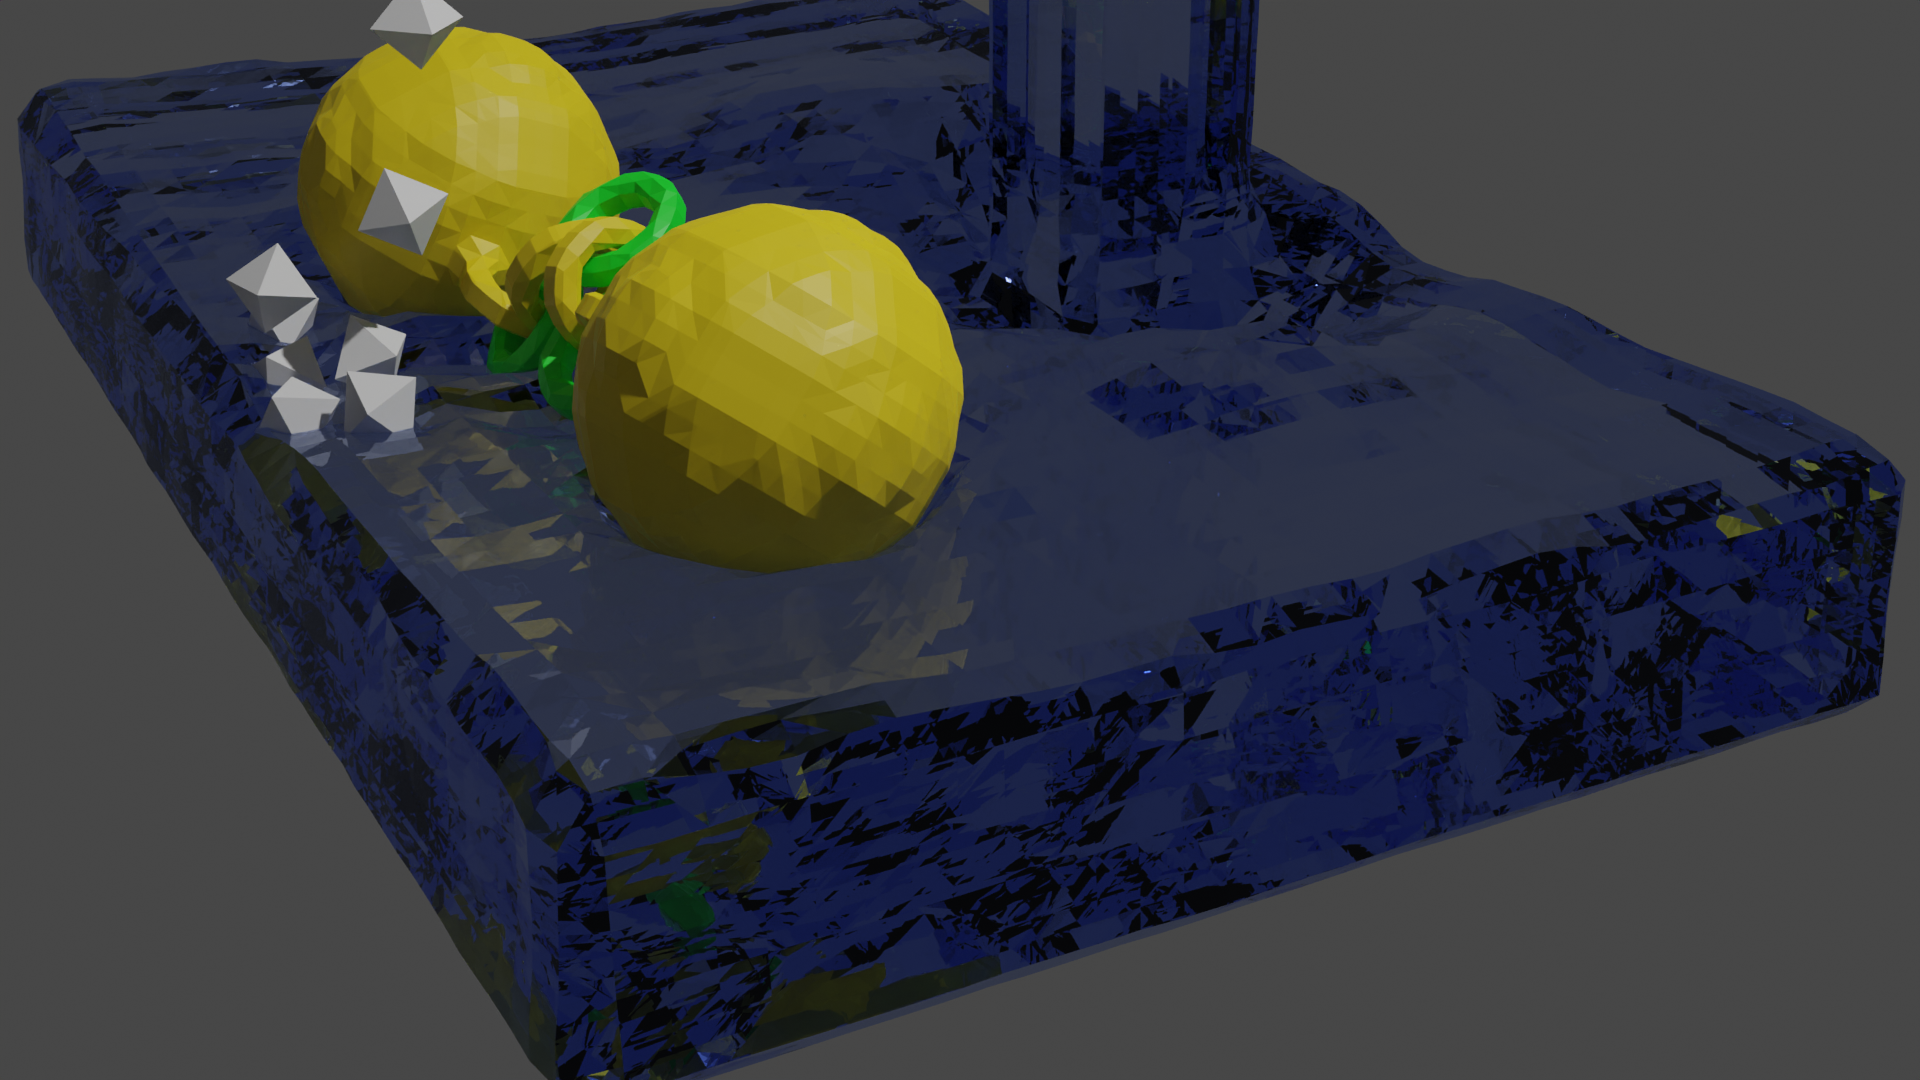
\includegraphics[width=0.4\textwidth]{../result/1.png}}
  \subfigure[]{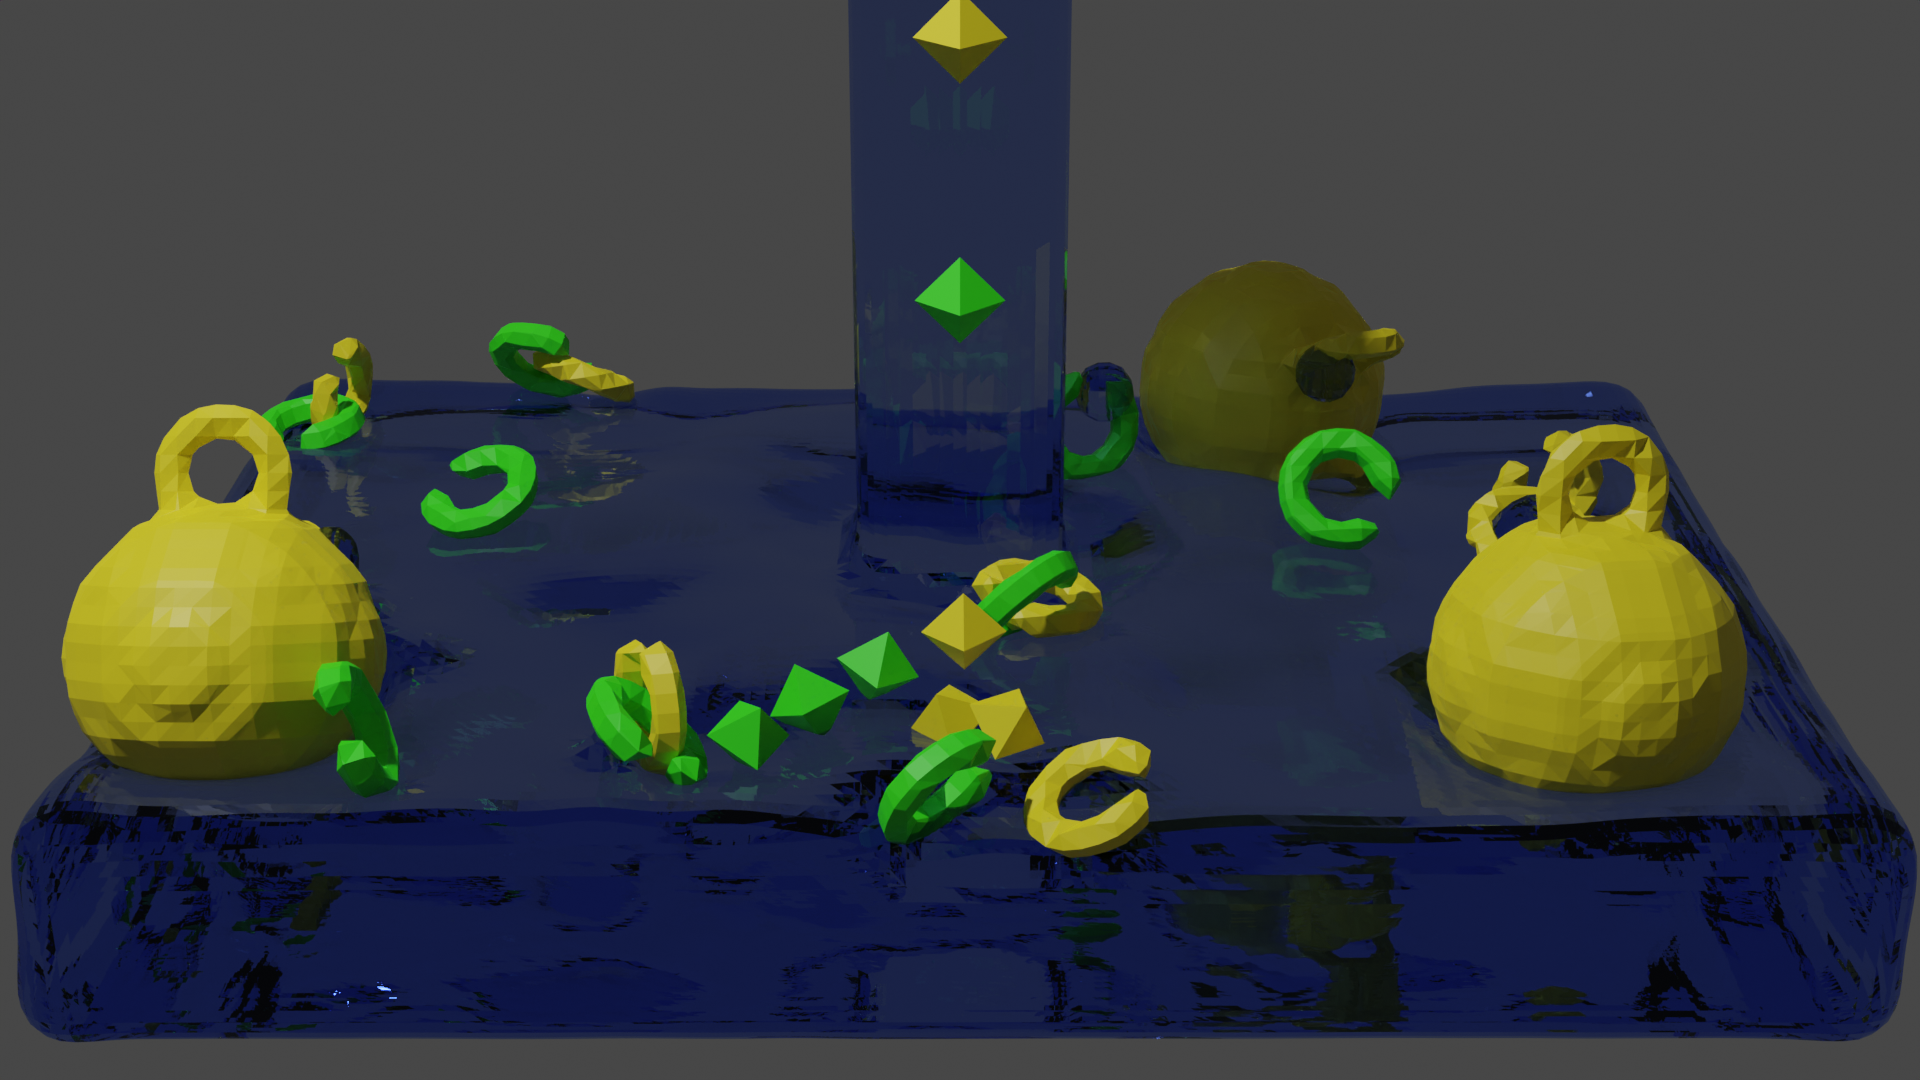
\includegraphics[width=0.4\textwidth]{../result/2.png}}
  \caption{two pictures chosen from the two videos}
\end{figure}

\subsection{Acceleration Ratio}
The acceleration effect of spatial grid method is obvious. Without it I can do nothing, so I don't test the 
exact acceleration ratio of it.
The acceleration effect of advanced numerical method is a little tricky. I will talk about it in section 5.1 Time Step.

The acceleration effect of GPU version is significant. But so far, 
I haven't been able to successfully achieve complete GPU acceleration, there are some weird issues. 
When running the first scene and the second scene, one issue the current $\texttt{sim\_gpu.cu}$ encountered is
the insufficient shared memory issue.
Specifically, section 3.3.2 mentions that when processing each grid, 
all 27 neighbor grids information will be loaded onto shared memory, 
greatly improving the efficiency of memory access. 
However, the particle density in these scenes is somewhat high, 
causing the data of 27 neighbor grids to be unable to be stored in the shared memory of a GPU block.

Nevertheless, I constructed the third scene, which is simpler than the first two scenes. 
This scene is only used for speed measurement, so I did not create the corresponding video.
This scene includes 86625 fluid particles and 50 output frames. Each frame requires 5 simulation steps. 
$\texttt{sim\_gpu.cu}$ works successfully in this scenario and runs at a quite fast speed. 
It only takes 6.8 seconds to run on a RTX 3090 I rented. As a comparison, on my PC whose CPU is
Intel(R)Core(TM) i7-8565U CPU @ 1.80GHz, the CPU version \texttt{sim.cu} takes 127.3 seconds to run.

\section{Discussion}

\subsection{Time Step}

One contribution of this paper\cite{2019TOG} is to propose a SPH solver for strong fluid-rigid coupling.
Its method differs from traditional weak fluid-rigid coupling methods like
the paper ``Versatile Rigid-Fluid Coupling for Incompressible SPH''\cite{AK2012}
%TODO: add citation
in the rigid body handling.
Weak fluid-rigid coupling method usually separately compute fluid motion and rigid body motion.
When computing fluid motion, the rigid body is regarded as a static obstacle. Then when handling rigid body,
the fluid-rigid interface forces are considered as a kind of pure external force like gravity, and rigid boddy motion
are handled by a separate rigid solver. However, in this paper, the 
computation of the acceleration of fluid and rigid body are interleaved in the
solver.

The paper claims that the most advantage of this strong fluid-rigid coupling method is stability so that 
it can use a much larger time step than weak fluid-rigid coupling method and achieve a better result.
I didn't implement weak fluid-rigid coupling method, so I can't empirically test this claim, and I don't 
know what kind of acceleration effect can this advanced method achieve in my scenes.
I only compare IISPH with the simple SPH solver using explicit integrator as showed in the presentation. 
The result shows that IISPH can indeed use a larger time step than the simple SPH solver and keep stable.

My experience is that the time step can not be too large yet even using this advanced method.
Too large time step causes weird penetration in the simulation. I think this is because the famous CFL condition\cite{Lewy1928}
%TODO: add citation
which provides an upper bound for the time step width, i.e.
\begin{align*}
  \Delta t \leq \lambda \frac{h}{\Vert v^{max}\Vert}
\end{align*}
where $\lambda$ is a constant, $h$ is the support radius(particles size), $\Vert v^{max}\Vert$ is the maximum velocity of particles.
Time step larger than this upper bound will make one particle move so far in one step that penetrates one layer of boundary particles.
The original paper also mentions this issue, "Another consequence of using
particles for the rigid-rigid contact handling is that their size and
velocity influence the maximum allowed time step due to the CFL
condition. However, this time step restriction generally applies for
particle-based boundary handling when the fluid is in contact with
a moving rigid body. Furthermore, in our scenes, the CFL condition
of the fluid solver normally dominated the time step." In my scenes, the CFL condition also seems to be the 
main bottleneck of increasing time step.

\subsection{Particle}

Another contribution of this paper is to propose a particle-based rigid solver using SPH pinciple.
Indeed, the SPH solver in this paper itself is also a feasibile rigid solver, though it's not the main purpose.
So an advantage of implementing SPH solver in this way is that 
fluid and rigid body simulations can be processed within the same framework. 
The same structure as the fluid can be used to store the particle representation of rigid bodies
 and handle collision detection between rigid bodies, 
 without the need for separately implemented rigid body mesh representation
 and rigid body collision detection in the solver or calling external rigid body solvers.
And the entire framework can easily adapt to different SPH fluid solvers and still support strong solid-liquid coupling.
Though I only implement IISPH as the foundation fluid solver, 
the original paper suggests that a large class of SPH fluid solvers can be used like IISPH, DFSPH, a solver for highly 
viscous SPH fluids\cite{VFSPH} and a solver for elastic SPH solids \cite{peer2018implicit}, 
%TODO: add citation
as long as this solver is iterative(can be written as the form required by the Main Algorithm \ref{MA} ).
\begin{figure}[h]
  \centering
  \subfigure[]{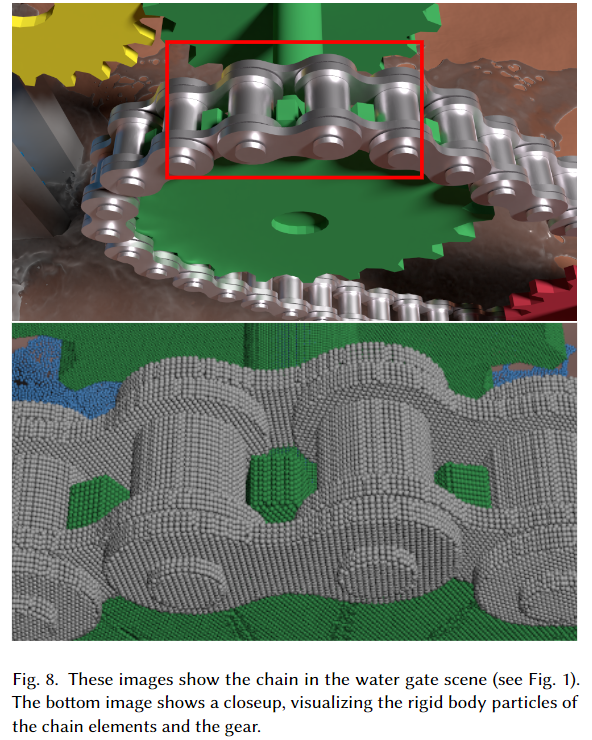
\includegraphics[width=0.3\textwidth]{3.png}}
  \subfigure[]{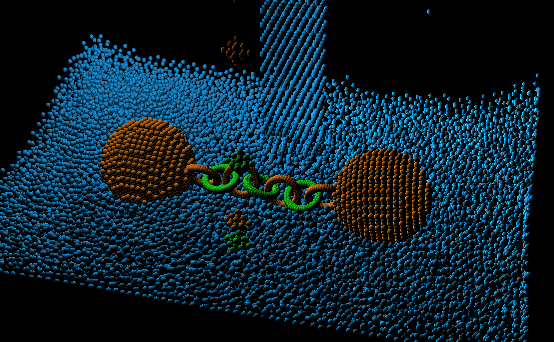
\includegraphics[width=0.5\textwidth]{4.png}}
  \caption{How the scene is represented by particles. The left is copied from the original paper. The right is from my scene.}
\end{figure}
\begin{figure}[h]
  \centering
  \subfigure[]{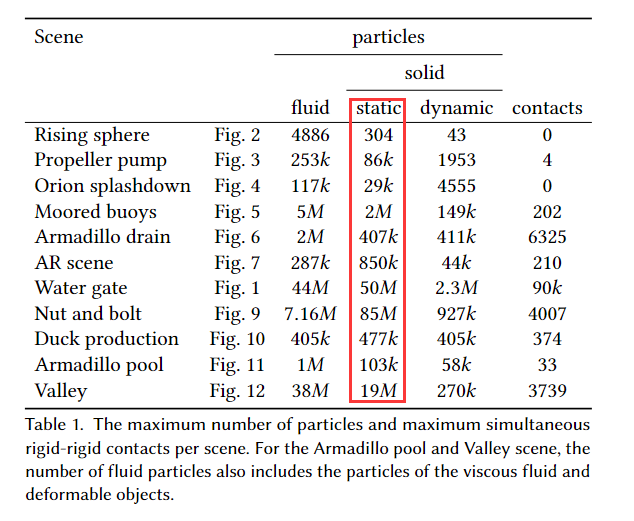
\includegraphics[width=0.5\textwidth]{5.png}}
  \caption{Note: Rising sphere is a two-dimensional case.}
\end{figure}

% At first, the circular rings in the scene were made of only one layer of particles.
% As the consequence, the rings are unnaturally penetrated in the simulation. 
% When I added more layers of particles, another issue arose. 
% Due to the thinness of the ring, multiple layers of particles are packed into a very narrow space, 
% resulting in an unnaturally high density and pressure of rigid particles in the ring. 
% Later, my solution was to use the correct Artificial rest volume computation 
% like the paper suggested
% % TODO: add citation
% instead of using the same radius as fluid particles for rigid particles.

However, particle representation 
also has some drawbacks. One has been mentioned in section 5.1 that particle representation subtly 
restricts the time step.
The second drawback is mentioned in section 3.4.2 that improving simulation performance needs increasing the number of particles.
One of its consequence is to decrease in simulation speed.
In my practice, static particles significantly slow down the simulation speed. 
A very practical problem I encountered during debugging is that I need to place many static solid particles on the spatial boundary 
to prevent dynamic solid/fluid particles from crossing the boundary as mentioned before. 
This results in dealing with a relatively high total number of particles even if 
only a small number of (dynamic) particles are used for simulation during debugging. 
Even in my final scenes, there are still over 30\% of particles that are static particles on the boundary. 
And it seems that this is not my own problem. 
In the original paper\cite{2019TOG}, 
% TODO: add citation
Table 1 also indicates that static solid particles are usually more than dynamic solid particles, 
and the number of static solid particles is usually on the same order of magnitude as fluid particles (except for the scene
"Rising sphere" which is a two-dimensional case).

The third drawback is that, this particle-based rigid handling doesn't match human intuition like direct rigid handling, and we 
do not know how to control rigid body interaction more precisely.
When coding, I merely have no intuition about what kind of rigid body interaction will my program performs.
As showed in the presentation, after finishing coding, I can eventually test my simulator and find that the collision
is almost elastic. Though I cannot guarantee that I have reproduced the simulator 100\% correctly, 
the paper doesn't mention how to control the elastic coefficient of rigid body collisions which is 
easy to control in traditional rigid body solvers. And it seems to be a difficult problem for a particle-based rigid solver.

% \section{External Tool}
% In this section, I list the external tools I used. 
% Though I didn't manually implement their funcionality, I still need to spend time finding them and learning how to use them.
% \begin{itemize}
%   \item Taichi: a programming language for high-performance computation on CPUs and GPUs. I use it as the render for debugging due to its high speed.
%   \item Splashsurf: a surface reconstruction tool. I use it to convert objects from particle representation to mesh representation as mentioned in section 3.2.
%   \item Blender: a 3D computer graphics software. I use it to render the final scenes with high quality.
% \end{itemize}

\section{Personal Feeling}

I mainly use C++ to implement the simulator on CPU. I also use CUDA to implement the GPU acceleration and use a little Python 
to render. I feel that the main drawback of my programming language tool chain is that it doesn't provide a good acceleration like Taichi.
Many of the problems I encountered during the debugging process required a significant amount of simulation computation to discover, because too 
few particles and too simple scenes can not expose these problems. Sometimes even increasing 
the amount of simulation computation is just the solution to the problem itself.
So the low efficiency of CPP+CPU greatly slowed down my debugging progress. 
Waiting for the end of a simulation lasting several tens of seconds took up a considerable portion of my debugging time.
During the process of project, I also considered using CUDA for GPU acceleration, 
but CUDA itself was very difficult to use and debug, which led me to not successfully completely implement the GPU version by now. 
It can be said that the GPU version did not provide me with any help in debugging and building the final scenes.
So, Taichi+GPU may be a better choice for faster debugging. 
Of course, my toolchain has indeed taught me some lower level things like different kinds of acceleration techniques and 
basic geometry operations which have been provided in the standard library of higheer-level languages, 
but the debugging process is indeed a bit painful.

My another feeling is that I also spent a lot of time searching and learning proper external tools throughout the entire project process. 
I have tried PBRT-v4 for fluid rendering, but there is a lack of good tutorials online, so I ultimately chose Blender. 
I also tried implement surface reconstruction by myself, but later found splashsurf. 
These tools are far away from the project topic, but they are necessary. 
From the perspective of improving the course experience for students,
I think that in future course design instructors can provide more basic introductions that can 
reduce unnecessary time consumption.



%%%%%%%%%%%%%%%%%%%%%%%%%%%%%%%%%%%%%%%%%%%%%%%%%%%%%%%%%%%%
{
    \small
    \bibliographystyle{plain} % We choose the "plain" reference style
	  \bibliography{main.bib}
}

\end{document}
\endinput
%%
%% End of file `sample-acmlarge.tex'.
